\documentclass[sigconf]{acmart}

\usepackage{graphicx}
\usepackage{algorithm} % for algorithms
\usepackage{algpseudocode}
\usepackage{booktabs} % For formal tables
\usepackage{amsthm} % For claims
\usepackage{bbm} % indicator function

% table
\usepackage[flushleft]{threeparttable} % http://ctan.org/pkg/threeparttable
\usepackage{booktabs,caption}

\theoremstyle{remark}

\settopmatter{printacmref=false, printccs=true, printfolios=true}
\pagestyle{empty} % removes running headers

\newcommand{\PicScale}{0.5}
\newcommand {\FlameStream} {FlameStream}
\begin{document}

\copyrightyear{2019} 
\acmYear{2019} 
\setcopyright{acmcopyright}
% \acmConference[BeyondMR'18]{Algorithms and Systems for MapReduce and Beyond }{June 15, 2018}{Houston, TX, USA}
% \acmBooktitle{BeyondMR'18: Algorithms and Systems for MapReduce and Beyond , June 15, 2018, Houston, TX, USA}
% \acmPrice{15.00}
% \acmDOI{10.1145/3206333.3209273}
% \acmISBN{978-1-4503-5703-6/18/06}

\title {Poster: reproducible and reliable distributed classification of text streams}

\author{Artem Trofimov,$^ {1,2}$    Mikhail Shavkunov,$^3$    Sergey Reznick,$^4$     Nikita Sokolov,$^{5}$   Mikhail Yutman,$^3$ \\   Igor E. Kuralenok,$^1$    and  Boris Novikov$^ {3}$ }
\affiliation{%
\institution{$^1$JetBrains Research}
}
\affiliation{%
\institution{$^2$Saint Petersburg State University}
}
\affiliation{%
\institution{$^3$National Research University Higher School of Economics}
}
\affiliation{%
\institution{$^4$ Kofax}
}
\affiliation{%
\institution{$^5$ ITMO University}
  \city{St. Petersburg} 
  \country{Russia}
}
\email{\string{trofimov9artem, mv.shavkunov, sergey.reznick, faucct, myutman, ikuralenok\string}@gmail.com, borisnov@acm.org}

\begin{abstract}

Large-scale classification of text streams is an essential problem that is hard to solve. Batch processing systems are scalable and proved their effectiveness for machine learning but do not provide low latency. On the other hand, state-of-the-art distributed stream processing systems are able to achieve low latency but do not support the same level of fault tolerance and determinism. In this work, we discuss how the distributed streaming computational model and fault tolerance mechanisms can affect the correctness of text classification data flow. We also propose solutions that can mitigate the revealed pitfalls.

\end{abstract}

\begin{CCSXML}
\begin{CCSXML}
\begin{CCSXML}
<ccs2012>
<concept>
<concept_id>10002951.10002952.10002953.10010820.10003208</concept_id>
<concept_desc>Information systems~Data streams</concept_desc>
<concept_significance>500</concept_significance>
</concept>
<concept>
<concept_id>10002951.10003317.10003347.10003356</concept_id>
<concept_desc>Information systems~Clustering and classification</concept_desc>
<concept_significance>500</concept_significance>
</concept>
<concept>
<concept_id>10002951.10003227.10003351.10003446</concept_id>
<concept_desc>Information systems~Data stream mining</concept_desc>
<concept_significance>300</concept_significance>
</concept>
</ccs2012>
\end{CCSXML}

\ccsdesc[500]{Information systems~Data streams}
\ccsdesc[500]{Information systems~Clustering and classification}
\ccsdesc[300]{Information systems~Data stream mining}

\keywords{Data streams, text classification, reproducibility, exactly once}

\maketitle

\thispagestyle{empty}

\section {Introduction}
\label {fs-short-intro}

Classification of large text streams is hard, but important task for researchers and practitioners. It has a wide range of applications including detection of emerging news and current user interests, suspicious traffic analysis, spam filtering, etc. Popular open-source libraries like sklearn~\cite{sklearn_api} and NLTK~\cite{bird2009natural} provide a rich set of tools, but they mostly aim at handling static datasets. The lack of scalability across multiple computational units is another limitation of these solutions. There are plenty of works which adapt batch processing systems for text classification~\cite{semberecki2016distributed, svyatkovskiy2016large, baltas2016apache}. Their advantages are fault tolerance, high throughput, and scalability. On the other hand, these systems do not provide low latency that is a strong requirement for most streaming applications.

An immediate idea is to employ a distributed stream processing engine such as Flink~\cite{Carbone:2017:SMA:3137765.3137777} or Storm~\cite{apache:storm}. However, stream processing systems have several important differences in comparison with batch engines: 

\begin{itemize}
    \item In a general case, failure and recovery are not transparent for a user. The guarantees on data in case of failures are defined in terms of delivery guarantees: {\em at least once} and {\em exactly once}. The choice of a guarantee may affect the correctness of text classification.
    \item Most of streaming systems are inherently non-deterministic. It means that different runs on the same data may produce different results. This feature can influence the classification process as well.
\end{itemize}

In this work, we investigate the applicability of state-of-the-art stream processing systems to the text classification and demonstrate the challenges that a developer can experience. Our study reveals issues similar to the problems mentioned by TFX project team~\cite{Baylor:2017:TTP:3097983.3098021} on machine learning at scale in general: reproducibility, reliability of results, fault tolerance, etc. For demonstration, we adapt text classification data flow that is typical for batch processing systems for state-of-the-art stream processing engine Apache Flink~\cite{Carbone:2017:SMA:3137765.3137777}. We show that failures within {\em at least once} guarantee may significantly shift the distribution of classification results. It is also indicated that races due to asynchronous channels in the data flow lead to a non-reproducible outcome. We demonstrate that straightforward solutions to the revealed issues may lead to performance overhead. More sophisticated approaches to solve the problems are touched upon.

The rest of the paper is structured as follows: the problem of text classification using stream processing engines and the typical data flow are discussed in section~\ref{fs-framework}, section~\ref{fs-discussion} contains the evaluation of the data flow on top of state-of-the-art stream processing system, approaches to get around the revealed issues are introduced in section~\ref{fs-solution}, prior works on the topic are mentioned in section~\ref{fs-related}, we discuss the results and our plans in~\ref{fs-conclusion}.

\section {Problem statement}
\label {fs-short-problem}

Let us consider the news topic classification as an illustration of a text stream multi-classification task. There are two input streams: pre-labeled and raw. The latter stream elements must be labeled by a classifier and delivered to end-user. The pre-labeled stream is used for updating a machine learning model with new data in order to adapt it to current events. The ultimate purpose is to achieve the distribution of news topics that is changing over time. This task is a typical representative of the text stream classification problem.

As the main requirement to a stream processing engine we claim the following: each output element must depend only on the input. In other words, node failures and execution environment parameters must not affect the results, similar to batch systems. Otherwise, it is hard to design a solution that provides reproducible and interpretable classification results.

\section {Data flow}
\label {fs-dataflow}

Typical classification pipeline based on bag-of-words text representation consists of three steps. The first one is computing TF-IDF features. The second one is training a classifier on these features or making a prediction. To adapt this pipeline for a stream processing engine, one needs to represent it in the form of a {\em logical graph}. It serves as a descriptive language for defining streaming computations. Vertices of a logical graph denote operations, while edges indicate data subscriptions between them. 

The initial point in our data flow is an {\em Source} vertex. It receives input texts from data producers and computes term frequencies. Computing of inverse document frequencies is a separate operation because it maintains a state and requires different data partitioning in a physical execution. {\em TF-IDF} vertex joins features corresponding to the same text and passes them to the {\em Text Classifier}. {\em Text Classifier} is the very last vertex that predicts a label and delivers it to a data consumer. The scheme of the proposed logical graph is shown in Figure~\ref{logical_graph}.

\begin{figure}[htbp]
  \centering
  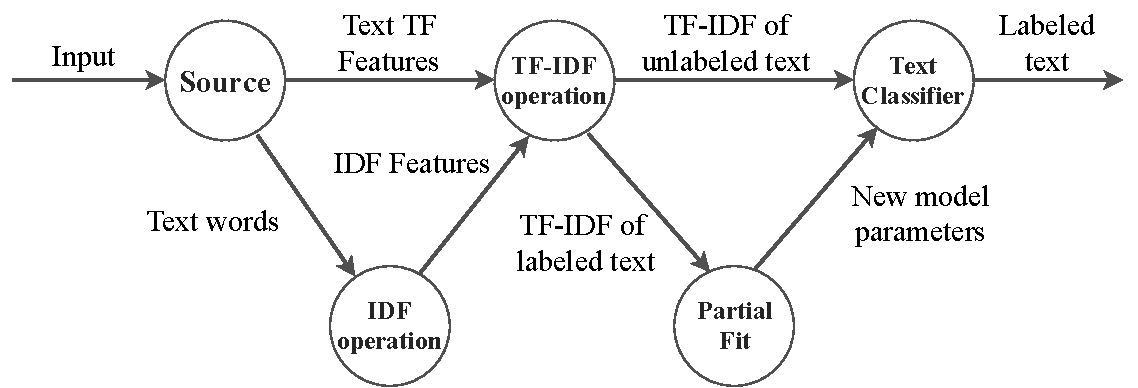
\includegraphics[scale=0.38]{pics/logical-graph}
  \caption{Text classification data flow}
  \label {logical_graph}
\end{figure}

Training pipeline is a separate branch within the logical graph introduced above. For already labeled text its features are sent to a {\em Partial fit} vertex instead of the {\em Classifier}. {\em Partial fit} vertex buffers all input elements until training is triggered. After training, the buffer flushes. Updated parameters of a machine learning model are saved for further training and broadcasted to all {\em Text Classifier} vertices.

\section {Challenges}
\label {fs-challenges}

\indent

{\bf Online training.} An issue regarding the pipeline is that the training process may be time-consuming. If training and prediction processes run consecutively, there will be significant latency spikes, e.g. if a training process lasts for several minutes, then spikes may be 10 000 times greater than latency for prediction. However, without synchronization, there will be no reproducible correspondence between texts and applied model. It is almost impossible to achieve the same results within a new run on the same data because the training time becomes a hidden parameter that influences output. For instance, assume that we make two runs. On the first run model update consumes 70 seconds, but on the second run 75 seconds due to extra CPU load. If training and predicting are not synchronized, more unlabeled input elements are processed by an outdated model in the second case, so the distribution of news topics may be different between these two runs. We propose two solutions for the issues in question:

\begin{itemize}
    \item Use online learning algorithms. In this case, model updating is smooth and its synchronization with training does not cause latency spikes.
    \item Consider model parameters as special input elements that are stored with other input elements in a persistent queue, e.g. using Kafka~\cite{kreps2011kafka}. To reproduce results, there is just a need to replay elements from this queue.
\end{itemize}

{\bf Delivery guarantees.} Requirements on reproducibility and predictability of classification results affect the choice of a delivery guarantee. If a stream processing system provides {\em at least once}, some input texts can be processed more than one time in case of failures. This behavior may lead to biased prediction results. For example, if a single sports article is processed many times due to multiple failures, the resulted topics distribution will show that sport is a hot news topic right now. Hence, the only suitable delivery guarantee is {\em exactly once}. The problem here is that it is hard to achieve both low latency (less than 500 ms) and exactly once. Table~\ref{comparison} shows if a state-of-the-art system supports both features. To the best of our knowledge, among open systems only~\FlameStream\ provides for both low latency and exactly once. This property is achieved using optimistic order enforcement that implies system-wide idempotence. The details of this approach are discussed in~\cite{we2018adbis, we2018beyondmr}.

\begin{table}[htbp]
\caption{Support of exactly and low latency (less than 500ms) by stream processing systems}
\begin{threeparttable}
\begin{tabular}{lcl}
System             & Exactly-once & Latency    \\
\hline
Storm,Heron,Samza  &    --         &   low            \\
Spark Streaming    &    +          &   high           \\
Flink              &    +          &   high$^*$       \\
MillWheel          &    +          &   NA             \\
FlameStream        &    +          &   low            \\
\end{tabular}
* with enabled exactly-once~\cite{we2018beyondmr}
\end{threeparttable}
\label{comparison}
\vspace{-6mm}
\end{table}

\section {Conclusion}
\label {fs-conclusion}

In this work, we investigated the suitability of distributed stream processing engines to the problem of text streams classification. We demonstrated that there are several pitfalls with an adaptation of data flow commonly used in batch systems for a stream processing:

\begin{itemize}
    \item Races in a physical data flow lead to irreproducible results: labels provided by a classifier may vary from run to run on the same test data. 
    \item Failures within {\em at least once} delivery guarantee can cause a biased distribution of classification results.
    \item Streaming data is rapidly changing, so there is a need to update the machine learning model on-the-fly. 
\end{itemize}

It was shown that straightforward solutions to the mentioned issues imply significant performance overhead. There were proposed potential solutions: to use~\FlameStream\ processing system with built-in determinism and efficient exactly once and to embed online learning into the data flow. 

As future work, we plan to implement a text classification framework that satisfies the following requirements:

\begin{itemize}
    \item Unbiased by distributed environment: node failures or races do not affect the ultimate result distribution.
    \item Reproducible: if input elements are stored in persistent storage, the same predictions are obtained on each new run.
    \item Concept drift conscious: changes in streaming data must be reflected in a machine learning model.  
\end{itemize}

\bibliographystyle{ACM-Reference-Format}
\bibliography{../../bibliography/flame-stream}

\end {document}

\endinput
